Wang Liping\\
Arocena Arezo Emiliano\\
Paredes Aguilera, Christian Limbert\\

\subsection*{\center Ejercicio 5C. Teoría del consumidor}
\vspace{1cm}

\subsubsection*{\center I. Describiendo los gustos individuales.}
\vspace{.5cm}

Invita a unos amigos a ver un partido en casa. Sus amigos quieren patatas fritas y cervezas, por lo que acude al supermercado donde existen dos tipos de mercancías: $‘$bolsas de patatas fritas$’$ (mercancía $1$) y $‘$latas de cerveza sueltas$’$ (mercancía $2$) (es decir, en el eje de abcisas vamos a indicar las patatillas y el de ordenadas las cervezas sueltas). En concreto, los gustos de sus amigos son tomar una bolsa de patatillas fritas por cada dos cervezas.\\\\

\begin{enumerate}[\large \bfseries 1.]

    %----------1.
    \item \textbf{¿Qué relación binaria caracteriza sus gustos con respecto a estas dos mercancías?}\\\\
	En primer lugar el conjunto de consumo viene dado por las patatas fritas y las cervezas, es decir, 

	\begin{tcolorbox}[colframe=white]
	$$\mathcal{X}^i = \lbrace x \in \mathbb{Z}^2 \; : \; x_l \geq 0 \; \mbox{para} \; l=1,2\rbrace.$$
	\end{tcolorbox}

	En segundo lugar, identificamos las cestas indiferentes.  

	Ya que las mercancías complementarias perfectas y dados los gustos de mis amigos de tomar una bolsa de patatas fritas por cada dos cervezas sueltas entonces nos será indiferente colocar en la cesta dos bolsas de patatas fritas y dos de cerveza o  una bolsa de patatas fritas y 4 de cerveza, como se ve a continuación,\\
    $$\left.\begin{array}{rcl} (2,2)&\succeq&(1,4) \\ (1,4) & \succeq&(2,2) \end{array}\right\}\Longrightarrow (2,2) \sim (1,4)$$\\
	Análogamente nos será indiferente tomar 3 bolsas de patatas fritas y 4 de cerveza ó 2 patatas fritas y 6 cervezas ya que los gustos de mis amigos serán tomar 2 patatas fritas y 4 cervezas sueltas.\\
	$$\left.\begin{array}{rcl} (3,4)&\succeq&(2,6) \\ (2,6) & \succeq&(3,4) \end{array}\right\}\Longrightarrow (3,4) \sim (2,6)$$\\
	Por lo tanto una cesta $x=(x_1,x_2)$ es indiferente a otra $y=(y_1,y_2)$ si, \\
	\begin{tcolorbox}[colframe=white]
	$$min\lbrace 2x_1,x_2\rbrace = min\lbrace 2y_1,y_2\rbrace$$
	\end{tcolorbox}

	Por ejemplo, se cumple la igualdad para $\mathcal{I}_2$,\\ $$min\lbrace 5\cdot 2 = 10, 4 \rbrace = min\lbrace 8,4 \rbrace =min\lbrace 6,4 \rbrace =min\lbrace 4, 4\rbrace = min\lbrace 2\cdot 2= 4,6 \rbrace =min\lbrace 4,8 \rbrace =min\lbrace 4,10\rbrace $$
	tal como se muestra en el gráfico siguiente,\\
	\begin{center}
	    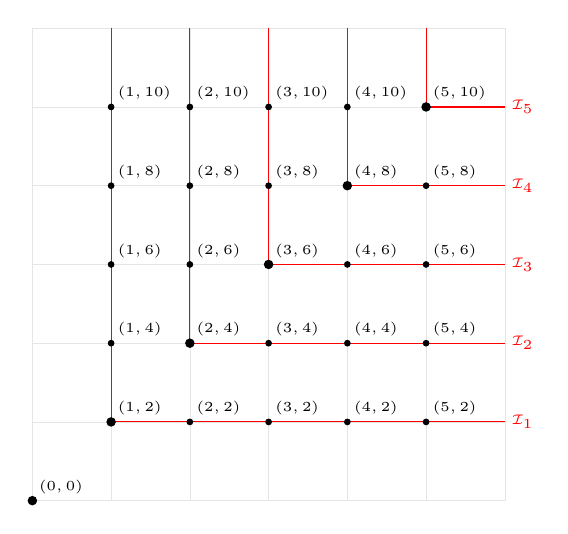
\begin{tikzpicture}
		% abscisa y ordenada
		\tkzInit[xmax= 5.5,xmin=0,ymax=11,ymin=0,ystep=2]
		\tiny\tkzLabelX[opacity=0.4,step=1, orig=false]
		\tiny\tkzLabelY[opacity=0.4,step=1, orig=false]
		% label x, f(x)
		\tkzDrawX[opacity= 1,label=Patatas fritas , right=.5]
		\tkzDrawY[opacity= 1,label=Latas de cervezas, below = -.5]
		%dominio y función
		\draw[step=1cm,black,very thin,opacity=.1] (0,0) grid (6,6);
		\draw[color=red](1,6)--(1,1)--(6,1);
		\draw[color=red](2,6)--(2,2)--(6,2);
		\draw[color=red](3,6)--(3,3)--(6,3);
		\draw[color=red](4,6)--(4,4)--(6,4);
		\draw[color=red](5,6)--(5,5)--(6,5);

		\filldraw[black] (0,0)node[above right]{$(0,0)$} circle (1.5pt);

		\filldraw[black] (5,1)node[above right]{$(5,2)$} circle (1pt);
		\filldraw[black] (4,1)node[above right]{$(4,2)$} circle (1pt);
		\filldraw[black] (3,1)node[above right]{$(3,2)$} circle (1pt);
		\filldraw[black] (2,1)node[above right]{$(2,2)$} circle (1pt);
		\filldraw[black] (1,1)node[above right]{$(1,2)$} circle (1.5pt);
		\filldraw[black] (1,2)node[above right]{$(1,4)$} circle (1pt);
		\filldraw[black] (1,3)node[above right]{$(1,6)$} circle (1pt);
		\filldraw[black] (1,4)node[above right]{$(1,8)$} circle (1pt);
		\filldraw[black] (1,5)node[above right]{$(1,10)$} circle (1pt);

		\filldraw[black] (5,2)node[above right]{$(5,4)$} circle (1pt);
		\filldraw[black] (4,2)node[above right]{$(4,4)$} circle (1pt);
		\filldraw[black] (3,2)node[above right]{$(3,4)$} circle (1pt);
		\filldraw[black] (2,2)node[above right]{$(2,4)$} circle (1.5pt);
		\filldraw[black] (2,3)node[above right]{$(2,6)$} circle (1pt);
		\filldraw[black] (2,4)node[above right]{$(2,8)$} circle (1pt);
		\filldraw[black] (2,5)node[above right]{$(2,10)$} circle (1pt);

		\filldraw[black] (5,3)node[above right]{$(5,6)$} circle (1pt);
		\filldraw[black] (4,3)node[above right]{$(4,6)$} circle (1pt);
		\filldraw[black] (3,3)node[above right]{$(3,6)$} circle (1.5pt);
		\filldraw[black] (3,4)node[above right]{$(3,8)$} circle (1pt);
		\filldraw[black] (3,5)node[above right]{$(3,10)$} circle (1pt);

		\filldraw[black] (5,4)node[above right]{$(5,8)$} circle (1pt);
		\filldraw[black] (4,4)node[above right]{$(4,8)$} circle (1.5pt);
		\filldraw[black] (4,5)node[above right]{$(4,10)$} circle (1pt);

		\filldraw[black] (5,5)node[above right]{$(5,10)$} circle (1.5pt);

		\draw[red](6,1)node[right]{$\mathcal{I}_1$};
		\draw[red](6,2)node[right]{$\mathcal{I}_2$};
		\draw[red](6,3)node[right]{$\mathcal{I}_3$};
		\draw[red](6,4)node[right]{$\mathcal{I}_4$};
		\draw[red](6,5)node[right]{$\mathcal{I}_5$};

	    \end{tikzpicture}
	\end{center}
	\vspace{.5cm}

	Por último caracterizamos formalmente los gustos a través de la relación binaria $"$ser como mínimo tan preferido como$"$ de la siguiente manera,\\
	\begin{tcolorbox}[colframe=white]
	\begin{center}
	    Dado cualquier par de cestas $x,y \in \mathcal{X}^i$ entonces $x \succeq^i y \; \Longleftrightarrow min\lbrace 2x_1,x_2 \rbrace \geq min\lbrace 2y_1, y_2\rbrace$.
	\end{center}
	\end{tcolorbox}
	\vspace{1cm}

    %----------2.
    \item \textbf{¿Puede representar sus gustos a través de conjuntos de indiferencia?}\\

	\begin{enumerate}[\bfseries (2.1)]

	    %----------(2.1)
	    \item Siendo que cumplen los axiomas de completitud y transitividad, tenemos que,\\
		\begin{tcolorbox}[colframe=white]
		$$x,y\in \mathcal{X}^i \; \mbox{entonces} \; x\succeq^i y \; \Longleftrightarrow \; min\lbrace 2x_1,x_2\rbrace \geq min\lbrace 2y_1,y_2\rbrace$$
		\end{tcolorbox}
		Luego y sabiendo que las ordenaciones serán consistente, es decir, que podemos identificar conjuntos de cestas indiferentes, podemos definirlas como, \\
		\begin{tcolorbox}[colframe=white]
		$$\mathcal{I}^i(x) = \lbrace y\in \mathcal{X}^i\; : \;  min\lbrace 2x_1,x_2 \rbrace = min\lbrace 2y_1, y_2 \rbrace \rbrace.$$
		\end{tcolorbox}
		Y por lo tanto, los gustos están representados por,\\
		\begin{tcolorbox}[colframe=white]
		$$\left(\mathcal{X}^i,\lbrace \mathcal{I}^i(x)\rbrace_{x\in \mathcal{X}^i}\right)$$
		\end{tcolorbox}
		\vspace{1cm}

	    %----------(2.2)
	    \item El gráfico de conjuntos indiferentes para $(1,2)$, $(2,4)$ y $(3,6)$ esta dado por,\\

	    \begin{center}
		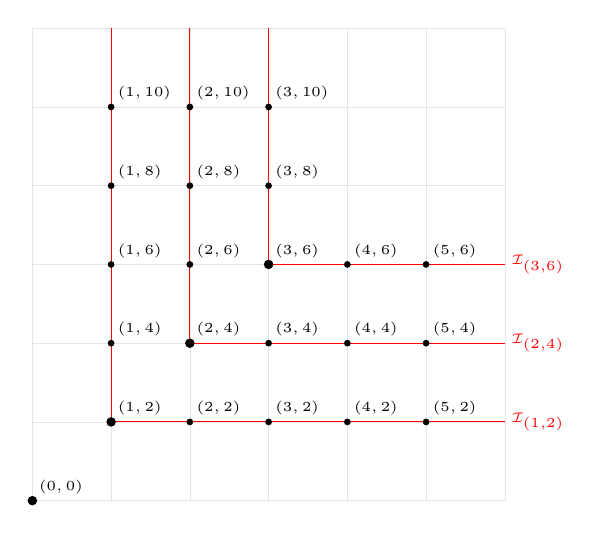
\begin{tikzpicture}
		    % abscisa y ordenada
		    \tkzInit[xmax= 5.5,xmin=0,ymax=11,ymin=0,ystep=2]
		    \tiny\tkzLabelX[opacity=0.4,step=1, orig=false]
		    \tiny\tkzLabelY[opacity=0.4,step=1, orig=false]
		    % label x, f(x)
		    \tkzDrawX[opacity= 1,label=Patatas fritas , right=.5]
		    \tkzDrawY[opacity= 1,label=Latas de cervezas, below = -.5]
		    %dominio y función
		    \draw[step=1cm,black,very thin,opacity=.1] (0,0) grid (6,6);
		    \draw[color=red](1,6)--(1,1)--(6,1);
		    \draw[color=red](2,6)--(2,2)--(6,2);
		    \draw[color=red](3,6)--(3,3)--(6,3);

		    \filldraw[black] (0,0)node[above right]{$(0,0)$} circle (1.5pt);

		    \filldraw[black] (5,1)node[above right]{$(5,2)$} circle (1pt);
		    \filldraw[black] (4,1)node[above right]{$(4,2)$} circle (1pt);
		    \filldraw[black] (3,1)node[above right]{$(3,2)$} circle (1pt);
		    \filldraw[black] (2,1)node[above right]{$(2,2)$} circle (1pt);
		    \filldraw[black] (1,1)node[above right]{$(1,2)$} circle (1.5pt);
		    \filldraw[black] (1,2)node[above right]{$(1,4)$} circle (1pt);
		    \filldraw[black] (1,3)node[above right]{$(1,6)$} circle (1pt);
		    \filldraw[black] (1,4)node[above right]{$(1,8)$} circle (1pt);
		    \filldraw[black] (1,5)node[above right]{$(1,10)$} circle (1pt);

		    \filldraw[black] (5,2)node[above right]{$(5,4)$} circle (1pt);
		    \filldraw[black] (4,2)node[above right]{$(4,4)$} circle (1pt);
		    \filldraw[black] (3,2)node[above right]{$(3,4)$} circle (1pt);
		    \filldraw[black] (2,2)node[above right]{$(2,4)$} circle (1.5pt);
		    \filldraw[black] (2,3)node[above right]{$(2,6)$} circle (1pt);
		    \filldraw[black] (2,4)node[above right]{$(2,8)$} circle (1pt);
		    \filldraw[black] (2,5)node[above right]{$(2,10)$} circle (1pt);

		    \filldraw[black] (5,3)node[above right]{$(5,6)$} circle (1pt);
		    \filldraw[black] (4,3)node[above right]{$(4,6)$} circle (1pt);
		    \filldraw[black] (3,3)node[above right]{$(3,6)$} circle (1.5pt);
		    \filldraw[black] (3,4)node[above right]{$(3,8)$} circle (1pt);
		    \filldraw[black] (3,5)node[above right]{$(3,10)$} circle (1pt);

		    \draw[red](6,1)node[right]{$\mathcal{I}_{(1,2)}$};
		    \draw[red](6,2)node[right]{$\mathcal{I}_{(2,4)}$};
		    \draw[red](6,3)node[right]{$\mathcal{I}_{(3,6)}$};

		\end{tikzpicture}
	    \vspace{1cm}

		    $\begin{tabular}{rcl}
			$\mathcal{I}^i(1,2)$&$=$&$\lbrace \ldots, (5,2),(4,2),(3,2),(2,2),(1,2),(1,4),(1,6),(1,8), (1,10),\ldots \rbrace$\\\\
			$\mathcal{I}^i(2,4)$&$=$&$\lbrace \ldots, (5,4),(4,4),(3,4),(2,6),(2,8),(2,10),\ldots\rbrace$\\\\
			$\mathcal{I}^i(3,6)$&$=$&$\lbrace \ldots,(5,6),(4,6),(3,6),(3,10), \ldots \rbrace$\\
		    \end{tabular}$\\
    
		    \end{center}
		\vspace{1cm}

	    %----------(2.3)
	    \item Según el capítulo 3 de Varian se menciona que, \begin{center}$"$las preferencias por los complementarios perfectos se caracterizan por el hecho de que la RMS no puede ser más que 0 o infinita$"$\end{center}
		En particular, y teniendo en cuenta los gustos de mis amigos. Si elegimos la curva de indiferencia $\mathcal{I}_{(2,4)}$ entonces la RMS será infinita porque mis amigos estarán dispuestos a renunciar cervezas por patatas fritas. De lo contrario, la RMS será cero ya que mis amigos no querrán cambiar cervezas por conseguir una bolsa más de patatas fritas.
		\vspace{1cm}

	\end{enumerate}

    %--------------------3.
    \item \textbf{¿Puede representar sus gustos a través de una función de utilidad?}\\

	\begin{enumerate}[\bfseries (3.1)]

	    %----------(3.1)
	    \item Para tal efecto necesitamos que a cada cesta se le asigne un número real de tal forma que se cumple el criterio de que si una cesta es indiferente a una segunda entonces le daremos el mismo valor numérico y si una cesta es estrictamente mas preferida que una tercera entonces se dará valores distintos. Se representa de la siguiente manera:     
		\begin{tcolorbox}[colframe=white]
		\begin{center}
		    \begin{tabular}{rccc|ccc}
			$u:$&$\mathcal{X}$ & $\longmapsto$ & $\mathbb{R}$ & $x \sim y$ & $\Rightarrow$ & $u(x)=u(y)$\\
			    & $x$ & $\longmapsto$ & $u(x_1,x_2)$ & $x\succ z$&$\Rightarrow$&$u(x)>u(z)$\\
		    \end{tabular}
		\end{center}
		\end{tcolorbox}
		\vspace{.3cm}
		Luego podríamos asignar dicha función de utilidad en función a la cantidad total de cervezas. 

		\begin{tcolorbox}[colframe=white]
		$$u(x_1,x_2)=min\lbrace 2x_1,x_2 \rbrace$$
		\end{tcolorbox}
		Por ejemplo

		\begin{center}
		    \begin{tabular}{cccccc}
			$u:$&$\mathcal{X}$&$\longmapsto$&$\mathbb{R}$&&\\
			 & $(x_1,x_2)$ & $\longmapsto$&$u(x_1,x_2)$&$=$&$min\lbrace 2x_1,x_2\rbrace$\\
			    & $(0,0)$ & $\longmapsto$ & $u(0,0)$ & $=$ & $0$\\
			    & $(2,2)$ & $\longmapsto$ & $u(2,2)$ & $=$ & $2$\\
			    & $(1,2)$ & $\longmapsto$ & $u(1,2)$ & $=$ & $2$\\
			    & $(1,4)$ & $\longmapsto$ & $u(1,4)$ & $=$ & $2$\\
			    & $(3,4)$ & $\longmapsto$ & $u(3,4)$ & $=$ & $4$\\
			    & $(2,4)$ & $\longmapsto$ & $u(2,4)$ & $=$ & $4$\\
			    & $(2,6)$ & $\longmapsto$ & $u(2,6)$ & $=$ & $4$\\
			    & $(4,6)$ & $\longmapsto$ & $u(4,6)$ & $=$ & $6$\\
			    & $(3,6)$ & $\longmapsto$ & $u(3,6)$ & $=$ & $6$\\
			    & $(3,8)$ & $\longmapsto$ & $u(3,8)$ & $=$ & $6$\\
		    \end{tabular}
		\end{center} 
		\vspace{1cm}

		%----------(3.2)
		\item Anteriormente para los cardinalistas, la función de utilidad que representaba las preferencias de un consumidor era única y  la representación de los gustos individuales de un consumidor en la teoría económica moderna es ordinalista es decir, se representan a través de una representación binaria que ordena cestas . Acá la cuestión es si existe una relación entre la herramienta de los cardinalistas (la función de utilidad) y la herramienta de los ordinalistas (relación de preferencias). \\
Dicho esto nos preguntamos que si para una representación de gustos a través de una relación de preferencias, existe una única función de utilidad o pueden existir más de una?. \\ 
A pesar del hecho que para los cardinalistas la función de preferencias de un consumidor era única, esta desapareció, por lo tanto la respuesta a esta cuestión es que no existe una única función de utilidad, es más existen infinitas funciones de utilidad, esto ya que al asignar números reales a cada preferencia, solo las asignamos por un propósito de ordenación que solo representan los gustos. \\\\

	    \end{enumerate}


\subsubsection*{\center II. Elección óptima.}
\vspace{.5cm}

    %-------------------4.
    \item \textbf{¿Cuál es la decisión óptima?.}\\\\
	Sus amigos han reunido $\overline{M} =12 \EUR$ (la renta). El precio de las patatillas fritas son $p_1 =1 \EUR$ y el de las cervezas sueltas es $p_2 =1 \EUR$; es decir, 
	$p = (p_1 , p_2 ) =$ $(1.00 \EUR$,  $1.00 \EUR $).\\

	\begin{enumerate}[\bfseries (4.1)]

	    %----------(4.1)
	    \item Sabiendo que los gustos de mis amigos son tomar una bolsa de patatas fritas por cada dos cervezas, entonces la cesta que elegiría sería la $(4,8)$, ya que querrán comer lo máximo en patatas como también cerveza en función a las preferencias mencionadas.\\\\ 

	    %----------(4.2)
	    \item El conjunto de consumo esta dado por,
		$$\mathcal{X} = \lbrace (p,c) \; /\; p,c > 0\rbrace,$$
		luego la renta y los precios están  dados por,
		\begin{center} $\overline{M} = 12 \EUR$ , $\qquad (\overline{p_1},\overline{p_2}) = (1,1)$, \end{center}
		por último el conjunto presupuestario será,
		$$\beta(\overline{p_1},\overline{p_2},\overline{M}) = \lbrace (p,c) \in \mathcal{X} \; /\; \overline{p_1}\cdot p + \overline{p_2}\cdot c \leq \overline{M}\rbrace.$$
		\vspace{.1 cm}

		\begin{center}
		    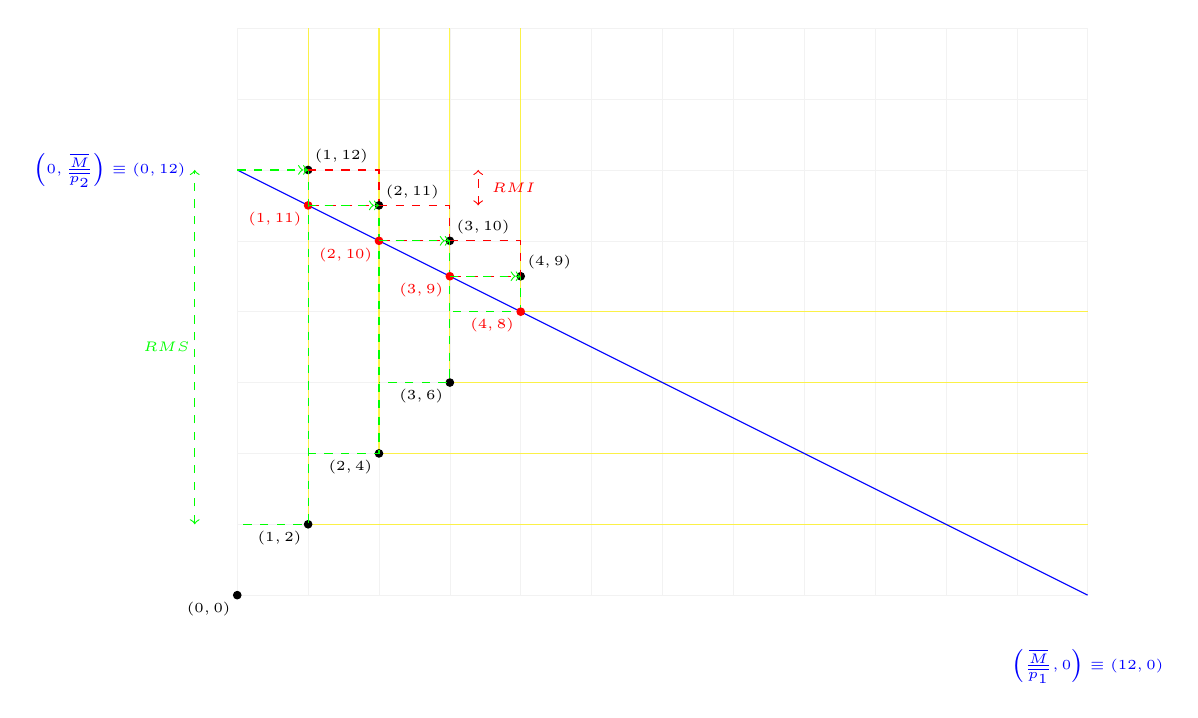
\begin{tikzpicture}[scale=.9]
			% abscisa y ordenada
			\tkzInit[xmax= 12.5,xmin=0,ymax=16.5,ymin=0,ystep=2]
			\tiny\tkzLabelX[opacity=0.4,step=1, orig=false]
			\tiny\tkzLabelY[opacity=0.4,step=1, orig=false]
			% label x, f(x)
			\tkzDrawX[opacity= 1,label=Patatas fritas (p), right=.1]
			\tkzDrawY[opacity= 1,label=Latas de cervezas (c), below = -.5]
			%dominio y función
			\draw[step=1cm,black,very thin,opacity=.05] (0,0) grid (12,8);

			\draw[color=yellow,opacity=.7](1,8)--(1,1)--(12,1);
			\draw[color=yellow,opacity=.7](2,8)--(2,2)--(12,2);
			\draw[color=yellow,opacity=.7](3,8)--(3,3)--(12,3);
			\draw[color=yellow,opacity=.7](4,8)--(4,4)--(12,4);

			\draw[opacity = 1,color=blue](12,0)--(0,6);

			\filldraw[black] (0,0)node[below left]{$(0,0)$} circle (1.5pt);
			\filldraw[black] (1,1)node[below left]{$(1,2)$} circle (1.5pt);
			\filldraw[black] (2,2)node[below left]{$(2,4)$} circle (1.5pt);
			\filldraw[black] (3,3)node[below left]{$(3,6)$} circle (1.5pt);



			\draw[blue](12,-1)node[]{$\left(\frac{\overline{M}}{\overline{p_1}},0\right)\equiv (12,0)$};
			\draw[blue](-1.8,6)node[]{$\left(0,\frac{\overline{M}}{\overline{p_2}}\right)\equiv (0,12)$};

			\filldraw[black] (1,6)node[above right]{$(1,12)$} circle (1.5pt);
			\filldraw[red] (1,5.5)node[below left]{$(1,11)$} circle (1.5pt);

			\draw[green,dashed](0,6)--(1,6)--(1,1)--(0,1);
			\draw[green, <->, dashed](-0.6,1)--(-0.6,6);
			\draw[green](-1,3.5)node[]{$RMS$};

			\draw[red,dashed](1,6)--(2,6)--(2,5.5)--(1,5.5);
			\draw[red, <->, dashed](3.4,5.5)--(3.4,6);
			\draw[red](3.9,5.75)node[]{$RMI$};

			\draw[green,dashed](1,5.5)--(2,5.5)--(2,2)--(1,2);
			\filldraw(2,5.5)node[above right]{$(2,11)$} circle (1.5pt);

			\draw[red,dashed](2,5.5)--(3,5.5)--(3,5)--(2,5);
			\filldraw[red] (2,5)node[below left]{$(2,10)$} circle (1.5pt);
			\filldraw(3,5)node[above right]{$(3,10)$} circle (1.5pt);

			\draw[green,dashed](2,5)--(3,5)--(3,3)--(2,3);
			\filldraw(4,4.5)node[above right]{$(4,9)$} circle (1.5pt);
			\draw[red,dashed](3,5)--(4,5)--(4,4.5)--(3,4.5);
			\filldraw[red] (3,4.5)node[below left]{$(3,9)$} circle (1.5pt);

			\draw[green,dashed](3,4.5)--(4,4.5)--(4,4)--(3,4);
			\draw[red,dashed](3,5)--(4,5)--(4,4.5)--(3,4.5);
			\filldraw[red] (4,4)node[below left]{$(4,8)$} circle (1.5pt);

			\draw[green,dashed,->>](0,6)--(1,6);
			\draw[green,dashed,->>](1,5.5)--(2,5.5);
			\draw[green,dashed,->>](2,5)--(3,5);
			\draw[green,dashed,->>](3,4.5)--(4,4.5);

		    \end{tikzpicture}
		\end{center}
		\vspace{1cm}


		Suponiendo que primero nos encontramos con el anaquel de las latas sueltas entonces nos preguntaremos si para $x$ cesta, 
		\begin{tcolorbox}[colframe=white]
		\begin{center}¿Debo meter una bolsa de patatas fritas en el carro?\end{center}
	    \end{tcolorbox}
		Para ello aplicamos la regla de decisión racional, conjuntamente con la relación marginal de sustitución $(RMS)$ y la relación marginal de intercambio $RMI = \dfrac{\overline{p_1}}{\overline{p_2}}$\\
		\vspace{.5cm}

			\begin{center}
			    \begin{tabular}{c|ccc}
				Cestas&$B(p)$&$>$&$C(p)$\\\\
				\hline\\
				$(0,12)$&$RMS=10$ & $>$ & $RMI=1$\\
				$(1,11)$&$9$ & $>$ & $1$\\
				$(2,10)$ & $7$ & $>$ & $1$\\
				$(3,9)$ & $4$ & $>$ & $1$ \\
				$(4,8)$ & $1$ & $=$ & $1$ \\
			    \end{tabular}
			    \vspace{1cm}
		    \end{center}

		    Por lo tanto ya que el beneficio es igual al coste, la elección optima estará dada por la cesta,\\
		    \begin{tcolorbox}[colframe=white]
			\begin{center}
			    $(4,8)$
			\end{center}
		    \end{tcolorbox}
		    \vspace{1cm}


	    %----------4.3.
		\item Sabiendo que los gustos de mis amigos son tomar una bolsa de patatas fritas por cada dos cervezas, y los precios vienen dados por $(\overline{p_1},\overline{p_2} = (2,1)$ entonces la cesta que elegirán será la $(3,6)$, ya que querrán comer lo máximo en patatas como también cerveza en función a las preferencias mencionadas.\\\\ 

	    Luego, el conjunto de consumo esta dado por,
		$$\mathcal{X} = \lbrace (p,c) \; /\; p,c > 0\rbrace,$$
		la renta y los precios están  dados por,
		\begin{center} $\overline{M} = 12 \EUR$ , $\qquad (\overline{p_1},\overline{p_2}) = (2,1)$, \end{center}
		por último el conjunto presupuestario será,
		$$\beta(\overline{p_1},\overline{p_2},\overline{M}) = \lbrace (p,c) \in \mathcal{X} \; /\; \overline{p_1}\cdot p + \overline{p_2}\cdot c \leq \overline{M}\rbrace.$$
		\vspace{.1 cm}

		\begin{center}
		    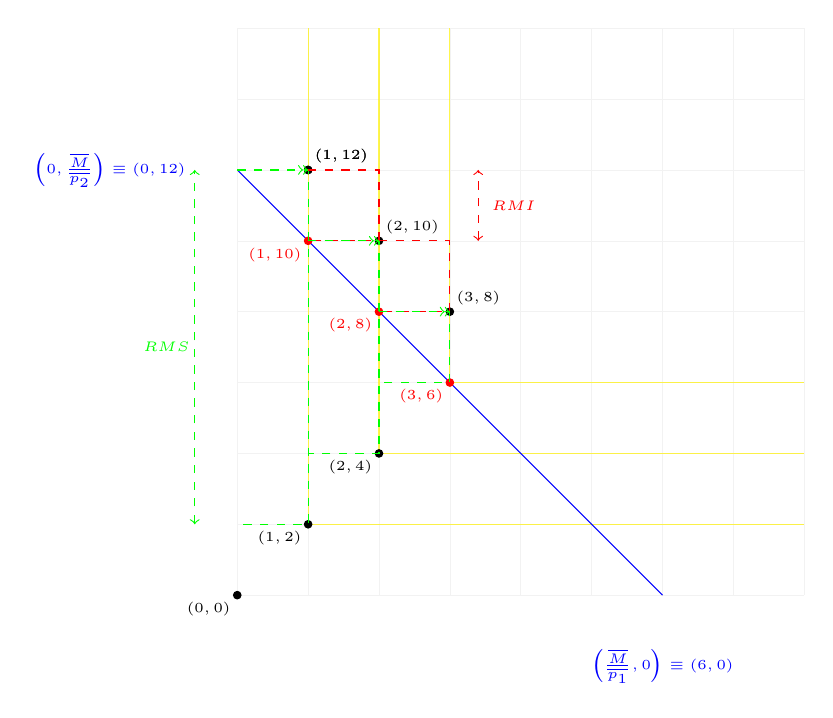
\begin{tikzpicture}[scale=.9]
			% abscisa y ordenada
			\tkzInit[xmax= 8.25,xmin=0,ymax=16.5,ymin=0,ystep=2]
			\tiny\tkzLabelX[opacity=0.4,step=1, orig=false]
			\tiny\tkzLabelY[opacity=0.4,step=1, orig=false]
			% label x, f(x)
			\tkzDrawX[opacity= 1,label=Patatas fritas (p), right=.1]
			\tkzDrawY[opacity= 1,label=Latas de cervezas (c), below = -.5]
			%dominio y función
			\draw[step=1cm,black,very thin,opacity=.05] (0,0) grid (8,8);

			\draw[color=yellow,opacity=.7](1,8)--(1,1)--(8,1);
			\draw[color=yellow,opacity=.7](2,8)--(2,2)--(8,2);
			\draw[color=yellow,opacity=.7](3,8)--(3,3)--(8,3);

			\draw[opacity = 1,blue](6,0)--(0,6);

			\filldraw[black] (0,0)node[below left]{$(0,0)$} circle (1.5pt);
			\filldraw[black] (1,1)node[below left]{$(1,2)$} circle (1.5pt);
			\filldraw[black] (2,2)node[below left]{$(2,4)$} circle (1.5pt);



			\draw[blue](6,-1)node[]{$\left(\frac{\overline{M}}{\overline{p_1}},0\right)\equiv (6,0)$};
			\draw[blue](-1.8,6)node[]{$\left(0,\frac{\overline{M}}{\overline{p_2}}\right)\equiv (0,12)$};

			\filldraw[black] (1,6)node[above right]{$(1,12)$} circle (1.5pt);

			\filldraw[red] (1,5)node[below left]{$(1,10)$} circle (1.5pt);
			\filldraw[red] (2,4)node[below left]{$(2,8)$} circle (1.5pt);
			\filldraw[red] (3,3)node[below left]{$(3,6)$} circle (1.5pt);

			\filldraw(1,6)node[above right]{$(1,12)$} circle (1.5pt);
			\filldraw(2,5)node[above right]{$(2,10)$} circle (1.5pt);
			\filldraw(3,4)node[above right]{$(3,8)$} circle (1.5pt);

			%lineas verdes
			\draw[green,dashed](0,6)--(1,6)--(1,1)--(0,1);
			\draw[green,dashed](1,5)--(2,5)--(2,2)--(1,2);
			\draw[green,dashed](2,4)--(3,4)--(3,3)--(2,3);

			%lineas rojas
			\draw[red,dashed](1,6)--(2,6)--(2,5)--(1,5);
			\draw[red,dashed](2,5)--(3,5)--(3,4)--(2,4);

			\draw[green, <->, dashed](-0.6,1)--(-0.6,6);
			\draw[green](-1,3.5)node[]{$RMS$};

			\draw[red, <->, dashed](3.4,5)--(3.4,6);
			\draw[red](3.9,5.5)node[]{$RMI$};

			\draw[green,dashed,->>](0,6)--(1,6);
			\draw[green,dashed,->>](1,5)--(2,5);
			\draw[green,dashed,->>](2,4)--(3,4);

		    \end{tikzpicture}
		\end{center}
		\vspace{1cm}

		Análogamente al anterior apartado primero nos encontramos con el anaquel de las latas sueltas entonces nos preguntaremos entonces nos preguntas si para $x$ cesta, 
		\begin{tcolorbox}[colframe=white]
		\begin{center}¿Debo meter una bolsa de patatas fritas en el carro?\end{center}
	    \end{tcolorbox}
		Para ello aplicamos la regla de decisión racional como también la relación marginal de sustitución $(RMS)$ y la relación marginal de intercambio $RMI = \dfrac{\overline{p_1}}{\overline{p_2}}$\\
		\vspace{.5cm}

			\begin{center}
			    \begin{tabular}{c|ccc}
				Cestas&$B(p)$&$>$&$C(p)$\\\\
				\hline\\
				$(0,12)$&$RMS=10$ & $>$ & $RMI=2$\\
				$(2,10)$&$8$ & $>$ & $2$\\
				$(3,8)$ & $6$ & $>$ & $2$ \\
				$(3,6)$ & $2$ & $=$ & $2$ \\
			    \end{tabular}
			    \vspace{1cm}
		    \end{center}

		    Por lo tanto ya que el beneficio es igual al coste, la elección optima  estará dado por la cesta,\\
		    \begin{tcolorbox}[colframe=white]
			\begin{center}
			    $(3,6)$
			\end{center}
		    \end{tcolorbox}
		    \vspace{1cm}


	    %----------- 4.4
		\item Suponiendo que los precios de las patatas fritas y las latas de cerveza sueltas son $$\overline{p}^{''} = \left( \overline{p_1}^{''},\overline{p_2}\right) = (4.00,1.00).$$ 
		    Entonces la cesta que eligirá es la cesta, 
		    \begin{tcolorbox}[colframe=white]
			$$(2,4)$$
		    \end{tcolorbox}
		    Luego podemos afirmar que la teoría económica puede explicar porque eligió la cesta $(2,4)$ a otra, fijándonos en los beneficios y costes de poder intercambiar un bien por otro bien  con un enfoque marginal.\\\\ 
		    


	\end{enumerate}

\subsubsection*{\center III. Curva de demanda.}
\vspace{.5cm}

    %--------------------5.
    \item \textbf{¿Cómo varía la decisión óptima cuando se modifica el conjunto presupuestario (cambios en precios o renta)?}
	\begin{center}
	    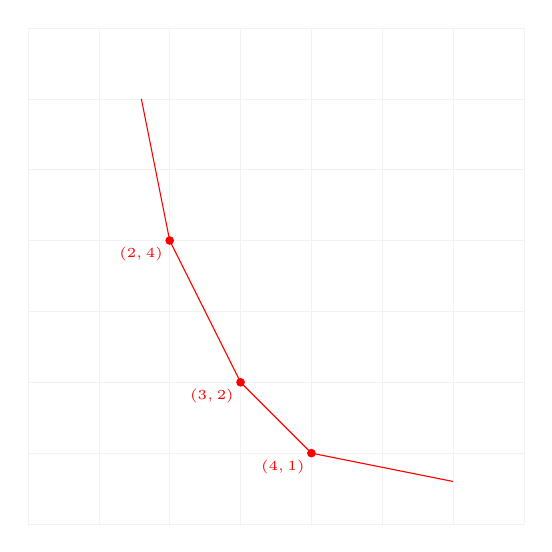
\begin{tikzpicture}[scale=.9]
		% abscisa y ordenada
		\tkzInit[xmax= 6.5,xmin=0,ymax=6.5,ymin=0,ystep=1]
		\tiny\tkzLabelX[opacity=0.4,step=1, orig=false]
		\tiny\tkzLabelY[opacity=0.4,step=1, orig=false]
		% label x, f(x)
		\tkzDrawX[opacity= 1,label=Patatas fritas (q), right=.1]
		\tkzDrawY[opacity= 1,label=Precio (p), below = -.5]
		%dominio y función
		\draw[step=1cm,black,very thin,opacity=.05] (0,0) grid (7,7);

		\filldraw[red](4,1)node[below left]{$(4,1)$} circle (1.5pt);
		\filldraw[red](3,2)node[below left]{$(3,2)$} circle (1.5pt);
		\filldraw[red](2,4)node[below left]{$(2,4)$} circle (1.5pt);

		\draw[red](1.6,6)--(2,4)--(3,2)--(4,1)--(6,0.6);


	    \end{tikzpicture}
	\end{center}
	\vspace{1cm}





\subsubsection*{\center IV. Cálculo analítico de la función de demanda.}
\vspace{.5cm}

    %--------------------6.
    \item \textbf{¿Cómo calcular analíticamente la cesta óptima y la función de demanda?}\\\\
	Suponga que las preferencias de un consumidor están representadas por la función de utilidad continua $u(x_1, x_2) = min\lbrace2x_1, x_2\rbrace$. Se pide:

	\begin{enumerate}[\bfseries a)]

	    %---------- a)
	    \item \textbf{Función de demanda.} El precio de las mercancías están dadas por $(p_1, p_2)$ y la renta del consumidor por $M$.\\\\
		Sean el conjunto de consumo, \\
		$$\mathcal{X} = \lbrace (x_1,x_2 \; / \; p \geq 0, c\geq 0 \rbrace,$$
		el conjunto presupuestario,\\ 
		$$\lbrace(x_1,x_2)\in \mathcal{X} \; / \; \overline{p_1}x_1 + \overline{p_2} x_2 \leq \overline{M}\rbrace$$
		y la función de utilidad \\
		$$u(x_1,x_2) = min\lbrace2x_1,x_2\rbrace$$\\
		entonces, el problema de consumidor estará dado por:\\
		\begin{tcolorbox}[colframe=white]
		$$\left\{\begin{array}{ccc}
			\max\limits_{x_1,x_2}&&u(x_1,x_2)=min\lbrace2x_1,x_2\rbrace\\\\
					     &s.a.&\begin{array}{rcl} \overline{p_1}x_1 + \overline{p_2}x_2&\leq &\overline{M}\\ x_1&\leq&0\\ x_2&\geq & 0 \end{array}\\\\
			   &dado&\overline{p_1},\overline{p_2},\overline{M}\\
		\end{array}\right.$$
		\end{tcolorbox}
		\vspace{1cm}

	    Ya que la función (Leontief) dada, no es derivable lo que se hará es igualar $x_1$ y $x_2$ como sigue:
	    
	    \begin{tcolorbox}[colframe=white]
		$$2x_1=x_2 \; \Longrightarrow \; x_1 = \dfrac{x_2}{2} \qquad (1)$$
	    \end{tcolorbox}
	    Sabiendo que los dos mercancías se consumen juntos, entonces supondremos que el consumidor gastará todo su dinero en un único bien cuyo precio será $\overline{p_1}+\overline{p_2}.$ Como se verá a continuación:\\
	    $$\overline{p_1}x_1 + \overline{p_2}x_2 =  \overline{M} \; \Longrightarrow \; \overline{p_1}\dfrac{x_2}{2} + \overline{p_2}x_2 =  \overline{M} \; \Longrightarrow \; x_2 = 2\left(\dfrac{\overline{M}}{p_1+2p_2}\right) \qquad (2)$$\\
	    Resolviendo análogamente para $x_1$,\\ 
	    $$\overline{p_1}x_1 + \overline{p_2}x_2 =  \overline{M} \; \Longrightarrow \; \overline{p_1}x_1 + 2\overline{p_2}x_1 = \overline{M} \; \Longrightarrow \; x_1 = \dfrac{\overline{M}}{p_1+2p_2}\qquad (3)$$\\
	    Luego por (1), (2) y (3) las funciones de demandas Marshallianas vienen dadas por:
	    \begin{tcolorbox}[colframe=white]
		$$x_1 = \dfrac{\overline{M}}{p_1+2p_2}$$
	    \end{tcolorbox}
	    \begin{tcolorbox}[colframe=white]
		$$x_2=2(x_1)$$
	    \end{tcolorbox}
	    \vspace{1cm}

	    %----------b)
	    \item \textbf{Elección óptima.} \\\\

		\begin{enumerate}[\bfseries b1)]

		    %-----b1
		    \item Precios $\overline{p} =  (\overline{p_1},\overline{p_2}) = (1.00,1.00)$ y renta $\overline{M} = 12$.\\\\

			Reemplazando en las funciones de demanda Marshallianas tenemos,\\
			$$x_1 = \dfrac{\overline{M}}{p_1+2p_2} = \dfrac{12}{1+2\cdot 1 } = 4 \qquad y \qquad x_2 = 2\left(x_1\right) = 2\left( 4 \right) = 8 $$\\\\
			de donde la cesta estará dada por,\\
			\begin{tcolorbox}[colframe=white]
			    $$(4,8)$$
			\end{tcolorbox}
			\vspace{1cm}


		    %-----b2
		    \item Precios $\overline{p}^{'} =  (\overline{p_1}^{'},\overline{p_2}) = (2.00,1.00)$ y renta $\overline{M} = 12$.\\\\

			Reemplazando en las funciones de demanda Marshallianas tenemos,\\
			$$x_1 = \dfrac{\overline{M}}{p_1+2p_2} = \dfrac{12}{2+2\cdot 1 } = 3 \qquad y \qquad x_2 = 2\left(x_1\right) = 2\left( 3 \right) = 6 $$\\\\
			de donde la cesta estará dada por,\\
			\begin{tcolorbox}[colframe=white]
			    $$(3,6)$$
			\end{tcolorbox}
			\vspace{1cm}

		    %-----b3
		    \item Precios $\overline{p}^{''} =  (\overline{p_1}^{''},\overline{p_2}) = (4.00,1.00)$ y renta $\overline{M} = 12$.\\\\

			Reemplazando en las funciones de demanda Marshallianas tenemos,\\
			$$x_1 = \dfrac{\overline{M}}{p_1+2p_2} = \dfrac{12}{4+2\cdot 1 } = 2 \qquad y \qquad x_2 = 2\left(x_1\right) = 2\left( 2 \right) = 4 $$\\\\
			de donde la cesta estará dada por,\\
			\begin{tcolorbox}[colframe=white]
			    $$(2,4)$$
			\end{tcolorbox}
			\vspace{1cm}

		\end{enumerate}

	    %----------c)
	    \item \textbf{Curvas de demanda}\\\\
		Sabiendo que la renta es $\overline{M}=12$ y los precios $\overline{p} =  (\overline{p_1},\overline{p_2}) = (1.00,1.00)$, $\overline{p}^{'} =  (\overline{p_1}^{'},\overline{p_2}) = (2.00,1.00)$ y $\overline{p}^{''} =  (\overline{p_1}^{''},\overline{p_2}) = (4.00,1.00)$ entonces la curva de demanda vendrá dada por, \\\\
		\begin{multicols}{2}
		\begin{center}
		    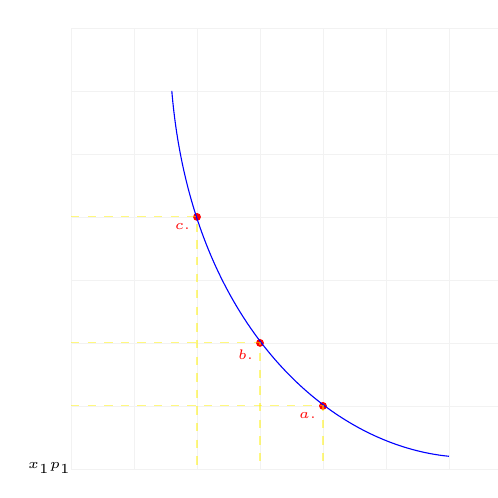
\begin{tikzpicture}[scale=.8]
			% abscisa y ordenada
			\tkzInit[xmax= 6.5,xmin=0,ymax=6.5,ymin=0,ystep=1]
			\tiny\tkzLabelX[opacity=0.4,step=1, orig=false]
			\tiny\tkzLabelY[opacity=0.4,step=1, orig=false]
			% label x, f(x)
			\tkzDrawX[opacity= 1,label=$x_1$, right=.1]
			\tkzDrawY[opacity= 1,label=$p_1$, below = -.5]
			%dominio y función
			\draw[step=1cm,black,very thin,opacity=.05] (0,0) grid (7,7);

			\filldraw[red](4,1)node[below left]{$a.$} circle (1.5pt);
			\filldraw[red](3,2)node[below left]{$b.$} circle (1.5pt);
			\filldraw[red](2,4)node[below left]{$c.$} circle (1.5pt);

			\draw[blue](1.6,6)..controls(1.9,2.4)and(4,0.4)..(6,.2);

			\draw[yellow,dashed,opacity=.5](0,4)--(2,4)--(2,0);
			\draw[yellow,dashed,opacity=.5](0,2)--(3,2)--(3,0);
			\draw[yellow,dashed,opacity=.5](0,1)--(4,1)--(4,0);

		    \end{tikzpicture}
		\end{center}
		\begin{center}
		    \begin{tabular}{c|ccccc}
			&cesta&$x_1$&$\overline{p_1}$&$\overline{p_2}$&$\overline{M}$\\
			\hline
			a.&(4,8)&4&1&1&12\\
			b.&(3,6)&3&2&1&12\\
			c.&(2,4)&2&4&1&12\\
		    \end{tabular}
		\end{center}
		\end{multicols}
		\vspace{1cm}

		Por otro lado, para $x_2$ y teniendo un mismo precio, se observará tres curvas de demanda desplazadas ya que dependen del precio del otro bien.\\\\

		\begin{multicols}{2}
		\begin{center}
		    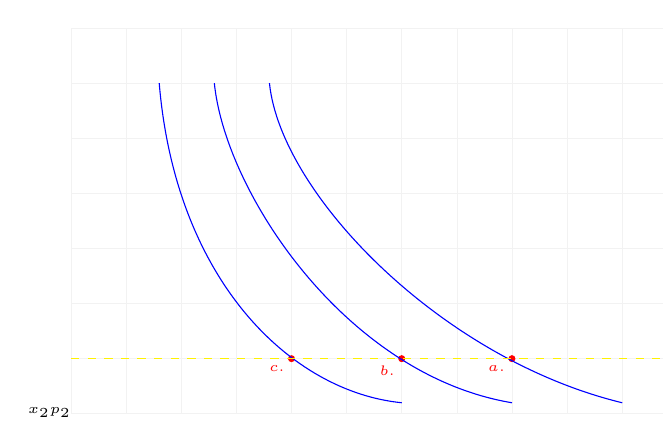
\begin{tikzpicture}[scale=.7]
			% abscisa y ordenada
			\tkzInit[xmax= 10.5,xmin=0,ymax=6.5,ymin=0,ystep=1]
			\tiny\tkzLabelX[opacity=0.4,step=1, orig=false]
			\tiny\tkzLabelY[opacity=0.4,step=1, orig=false]
			% label x, f(x)
			\tkzDrawX[opacity= 1,label=$x_2$, right=.1]
			\tkzDrawY[opacity= 1,label=$p_2$, below = -.5]
			%dominio y función
			\draw[step=1cm,black,very thin,opacity=.05] (0,0) grid (11,7);

			\filldraw[red](4,1)node[below left]{$c.$} circle (1.5pt);
			\filldraw[red](6,1)node[below left]{$b.$} circle (1.5pt);
			\filldraw[red](8,1)node[below left]{$a.$} circle (1.5pt);

			\draw[blue](1.6,6)..controls(1.9,2.4)and(4,0.4)..(6,.2);
			\draw[blue](2.6,6)..controls(2.8,4)and(5,.7)..(8,.2);
			\draw[blue](3.6,6)..controls(3.8,4)and(6.7,1)..(10,.2);

			\draw[yellow,dashed,opacity=1](0,1)--(11,1);

		    \end{tikzpicture}
		\end{center}
		\begin{center}
		    \begin{tabular}{c|ccccc}
			&cesta&$x_2$&$\overline{p_2}$&$\overline{p_1}$&$\overline{M}$\\
			\hline
			a.&(4,8)&8&1&1&12\\
			b.&(3,6)&6&1&2&12\\
			c.&(2,4)&4&1&4&12\\
		    \end{tabular}
		\end{center}
	    \end{multicols}
		\vspace{1cm}


	    %----------d)
	    \item \textbf{Función indirecta de utilidad}\\\\
		Definiendo la función indirecta de utilidad se tiene que 
		$$u(x_1,x_2) = min\lbrace \alpha x_1,\beta x_2\rbrace$$
		entonces,
		$$x_1=\dfrac{\overline{M}}{\overline{p_1}+\frac{\alpha}{\beta}\overline{p_2}}, \qquad x_2=\dfrac{\overline{M}}{\frac{\beta}{\alpha}\overline{p_1}+\overline{p_2}}$$
		así remplazando en la función de utilidad obtenemos,
		$$\mathcal{V}(\overline{p},\overline{m}) = min \left\{ \dfrac{\alpha \overline{M}}{\overline{p_1} + \dfrac{\alpha}{\beta}\overline{p_2}},\dfrac{\beta \overline{M}}{\dfrac{\beta}{\alpha}\overline{p_1}+\overline{p_2}} \right\} = min \left\{ \dfrac{\dfrac{\alpha}{\alpha} \overline{M}}{\dfrac{\overline{p_1}}{\alpha} + \dfrac{\alpha}{\beta}\dfrac{\overline{p_2}}{\alpha}},\dfrac{\dfrac{\beta}{\beta} \overline{M}}{\dfrac{\beta}{\alpha}\overline{p_1}+\dfrac{\overline{p_2}}{\beta}} \right\} = min \left\{ \dfrac{\overline{M}}{\dfrac{\overline{p_1}}{\alpha} + \dfrac{\overline{p_2}}{\beta}},\dfrac{\overline{M}}{\dfrac{\overline{p_1}}{\alpha}+\dfrac{\overline{p_2}}{\beta}} \right\}$$
		observamos que las ecuaciones son las mismas y por lo tanto,\\
		$$\mathcal{V}(\overline{p},\mathcal{M}) = \dfrac{\overline{M}}{\dfrac{\overline{p_1}}{\alpha}+\dfrac{\overline{p_2}}{\beta}}$$\\\\
		Luego de manera particular, sabiendo que la función de utilidad viene dada por 
		$$min\lbrace 2x_1,x_2\rbrace$$
		entonces la función indirecta de utilidad será 

		\begin{tcolorbox}[colframe=white]
		    $$\mathcal{V}(\overline{p},\overline{M}) = \dfrac{\overline{M}}{\dfrac{\overline{p_1}}{2}+\overline{p_2}} = \dfrac{2\overline{M}}{2\overline{p_2}+\overline{p_1}}$$
	    \end{tcolorbox}



	\end{enumerate}


\end{enumerate}
